\chapter{Architektura}

Emulátor jakéhokoliv hardwarového systému je ve své podstatě velmi komplexní,
proto je třeba správě rozvrhnout celkovou implementaci tohoto projektu. 
Zaprvé, je třeba myslet na udržitelnost kódu a schopnost jej bez větších problémů rozšiřovat a
za druhé, komplexita kódu by měla být dělitelná do jednotlivých jednotek.

Emulátor také potřebuje přístup k oknu a být schopen vykreslovat obsah grafické paměti
na obrazovku.

\section{Nástroje}

Pro tyto účely a požadavky jsem zvolil \textit{C++} jakožto jazyk pro implementaci.
\textit{Objektivně orientovaný} přístup k designu projektu a \textit{polymorfismus} tohoto jazyka
je pro tento projek ideální.

Pro přístup ke grafickému rozhranní jsem zvolil knihovnu \textit{SDL2}, což je univerzální
nástroj pro otevírání okna v operačním systému a mýt schopnost do něj kreslit.
\textit{SDL2} mimo jiné také umožňuje práci s obrázky a hudbou.

\section{Hardwarová komponenta}

\textit{PlayStation} ve svém hardwarovém designu připomíná velice obyčejný počítač, kterému byly
odstraněny přebitečné komponenty.

\textit{Sony}, narozdíl od svých oponentů, vytvořilo tuto konzoli z relativně dobře 
dokumentovaných čipů již existujících počítačů. Samozřejmě \textit{PlayStation} obsahuje i
patentované, na míru udělané součástky, které se snaží ulehčit práci procesoru.

Tyto hardwarové čipy sdílejí velmi podobné rozhranní. To je dáno tím faktem, že 
\textit{PlayStation} je nadesignován jako \textit{Memory-mapped I/O}. To znamená, že
sběrnice systému má uniformní paměťové rozložení, přičemž jednotlivé komponenty se mapují
do specifických paměťových intervalů. Jednotlivé komponenty pak mohou do těchto intervalů zapisovat nebo číst
a sběrnice pak rozdistribuuje tyto přístupy daným komponentám.

Díky tomuto faktu každá hardwarová komponenta musí mít následující schopnosti:

\begin{itemize}
    \item{\textit{Reset/Inicializace} komponenty}
    \item{\textit{Čtení} z komponenty}
    \item{\textit{Zápis} do komponenty}
    \item{Provedení \textit{jednotky práce} dané komponenty}
\end{itemize}

Pomocí dědičnosti a virtuálních metod \textit{C++} můžeme specifikovat virtuální třídu,
která bude sloužit jako báze pro všechny hlavní hardwarové komponenty.

\begin{figure}[hbt]
	\centering
	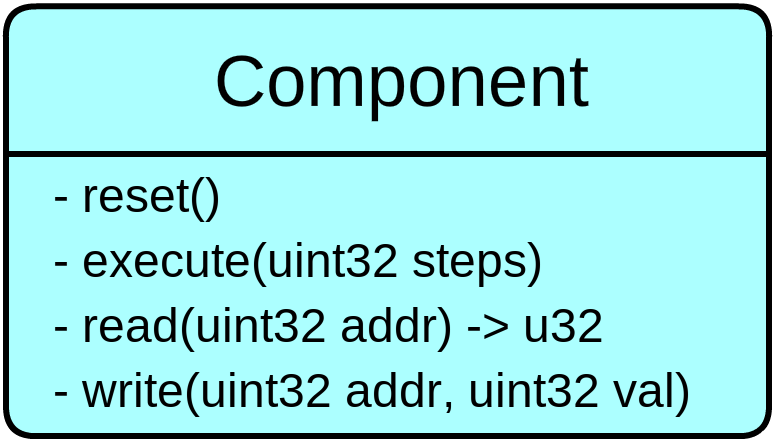
\includegraphics[width=0.4\textwidth]{obrazky-figures/component.png}
	\caption{Rozhranní, které každá hardwarová komponenta musí respektovat.}
	\label{component}
\end{figure}

\section{Návrh architektury}

\textit{PlayStation} se dělí na několik hlavních hardwarových komponent. Jsou to:

\begin{itemize}
    \item{Sběrnice}
    \item{Central Processing Unit \textbf{(CPU)}}
    \item{Graphics Processing Unit \textbf{(GPU)}}
    \item{Sound Processing Unit \textbf{(SPU)}}
    \item{3 Časovače/Hodiny}
    \item{Ovladač přerušení}
    \item{Ovladač přímého přístupu do paměti \textbf{(DMA)}}
    \item{Dekodér makrobloku \textbf{(MDEC)}}
    \item{CD-ROM}
\end{itemize}

Každá z těchto komponent je důležitá pro správné fungování emulátoru jako celku.
Jednotlivé propojení komponent a schopnost kdo s kým může komunikovat je popsáno v celkovém návrhu.

\begin{figure}[hbt]
	\centering
	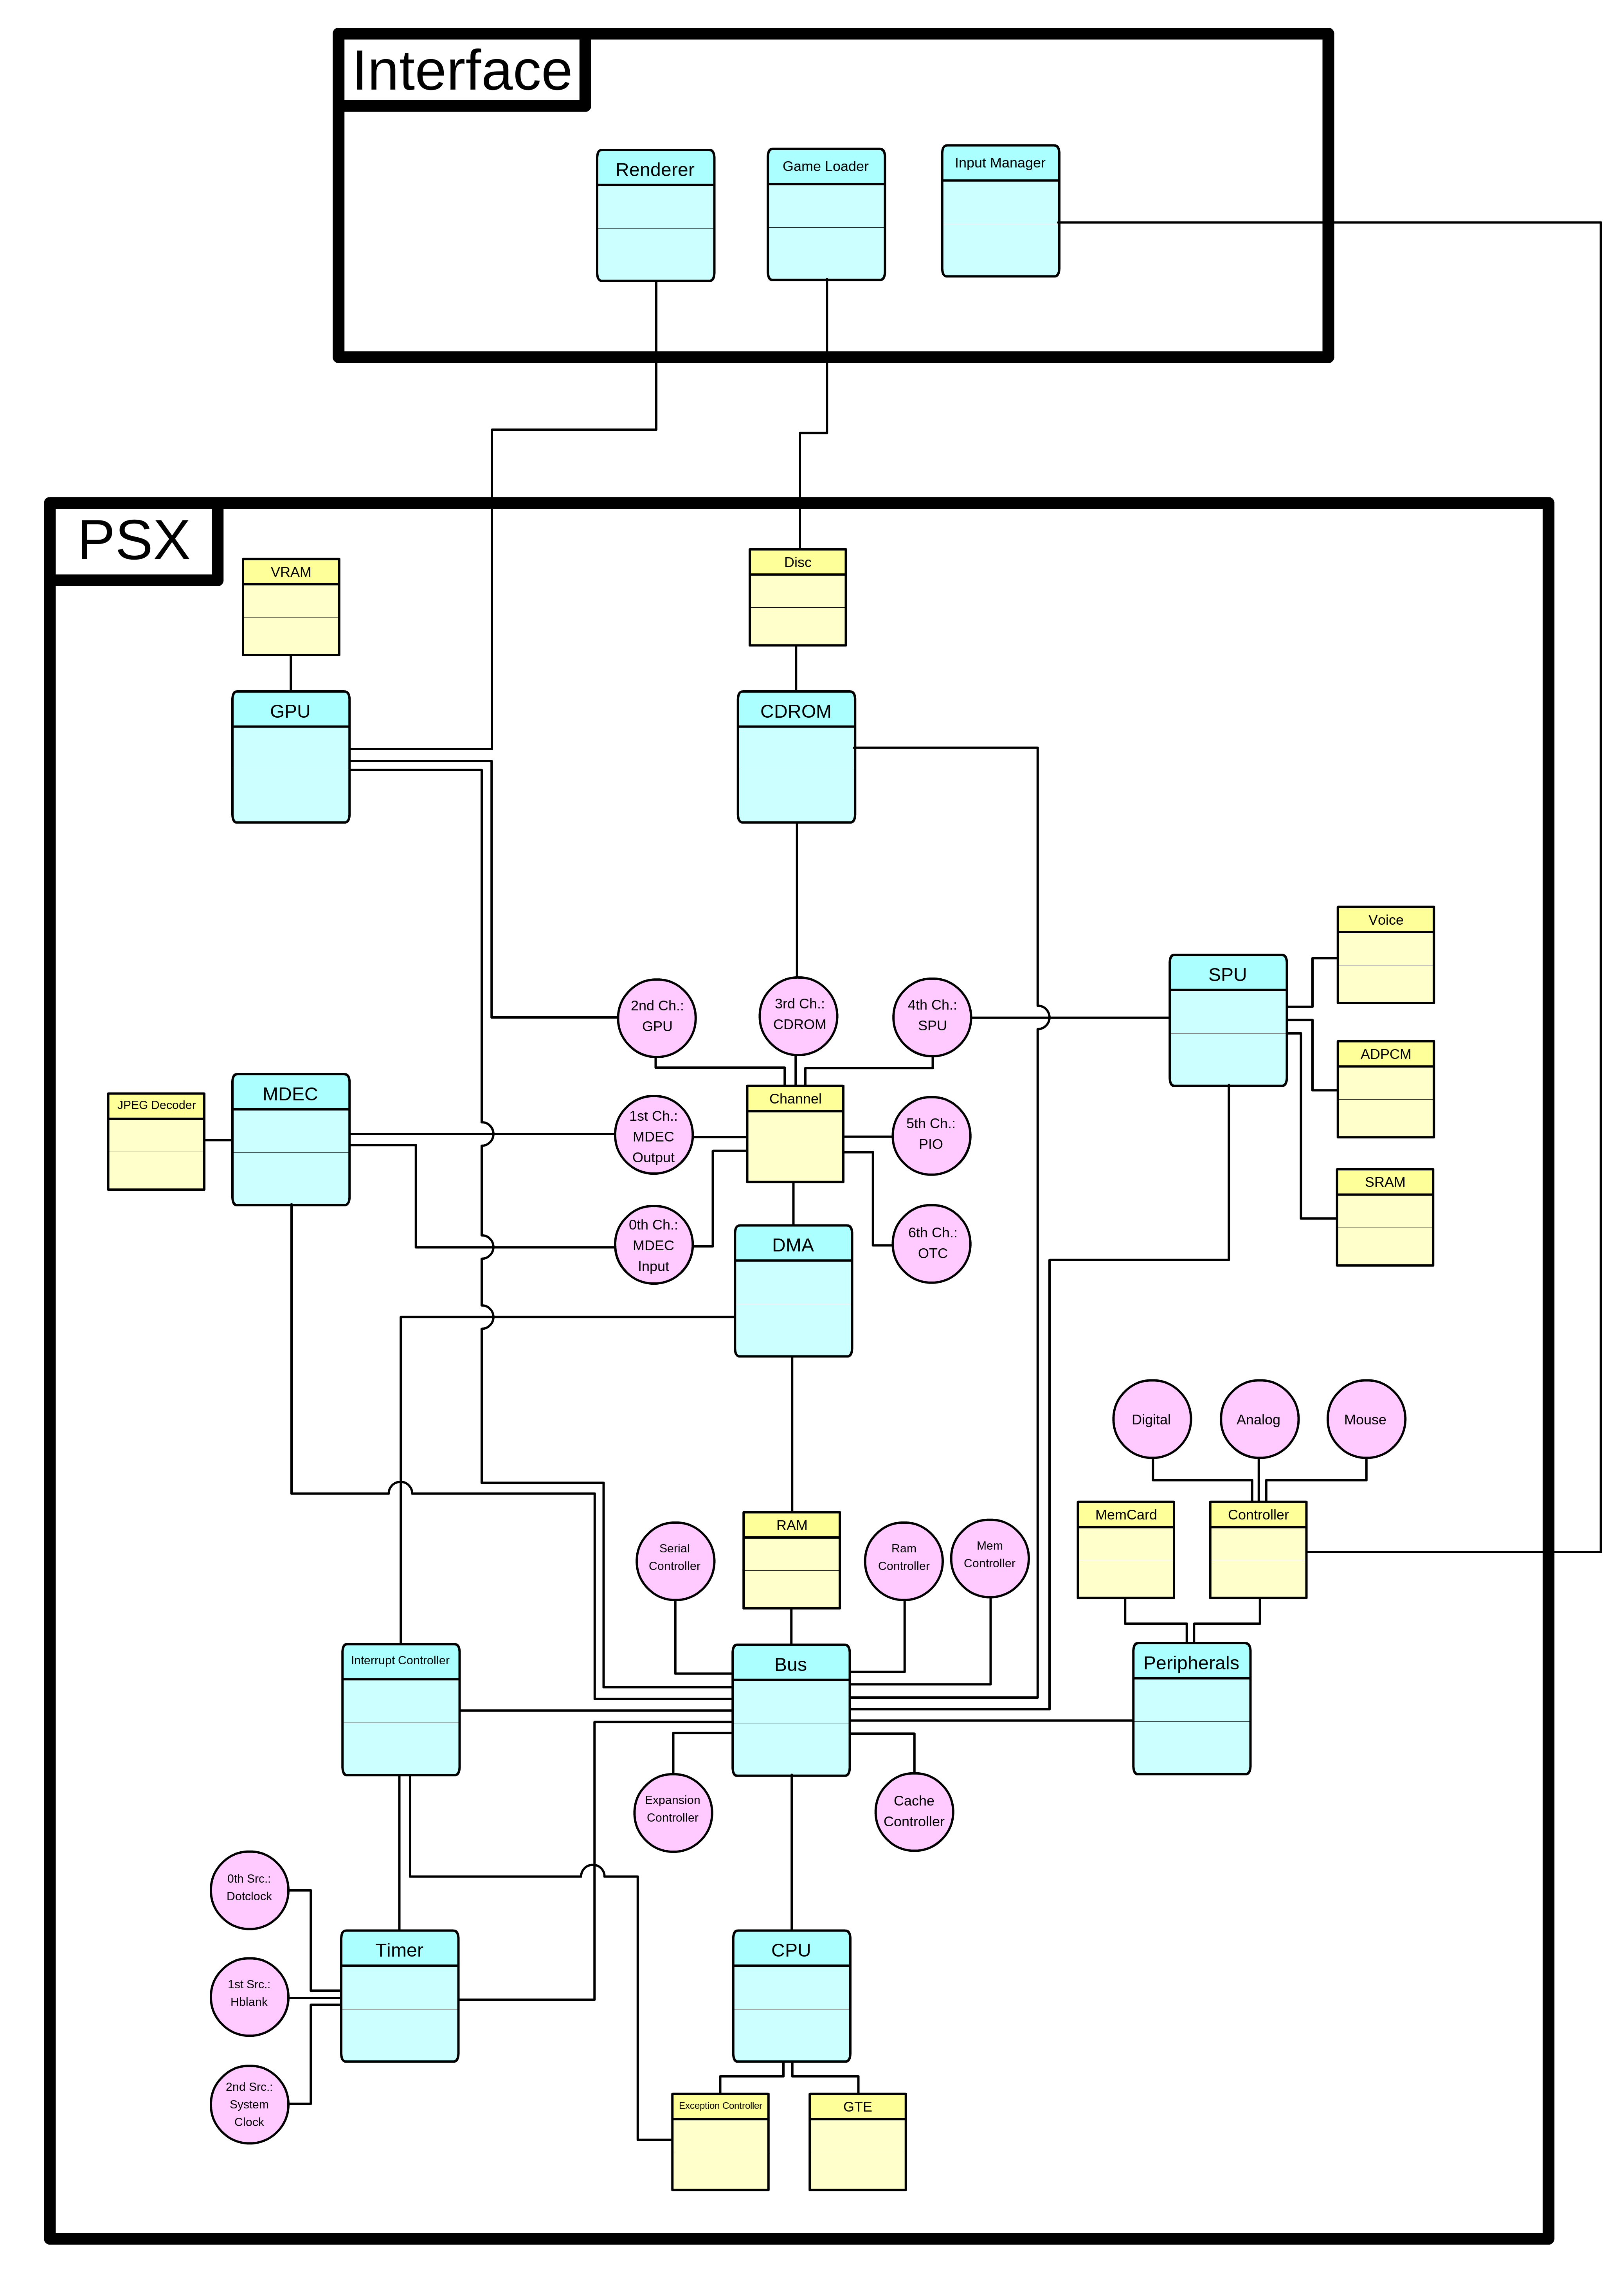
\includegraphics[width=1.0\textwidth]{obrazky-figures/psx-layout.png}
	\caption{Kompletní návrh zapojení nejenom hardwarových komponent emulátoru, ale i nadstavby nutné pro zpřístupnění stavu konzole.}
	\label{psx-layout}
\end{figure}

V návrhu jsou také reflektovány podřadné komponenty, které nemohou fungovat samostatně.
toto se například týká komponenty \textit{Geometry Transformation Engine (GTE)}, což je
ko-procesor starající se o práci s lineární algebrou. Jelikož k této komponentě lze přistoupit
pouze skrz \textit{CPU} pomocí speciální instrukce, nelze chápat tuto komponentu jako samostaný celek.

Každá komponenta je pak propojena se sběrnicí, kvůli \textit{Memory-mapped I/O}. Existují
i ovšem přímá propojení, bez sběrnice jako prostředníka. To je hlavně díky \textit{DMA} komponentě,
která se stará o rychlý přenos dat, aniž by se \textit{CPU} o tento přenos staralo. Další
přímá propojení jsou kvůli správě přerušení. Vzhledem k tomu, že přerušení může nastat skoro v
každé komponentě, je nutné toto přerušení propagovat do \textit{Ovladače vyjímek}, který pak
upraví stav \textit{CPU} a přerušení se následně zpracuje jako výjimka.
